\documentclass{article}

% Required packages (merged from hw5_template.tex and hw6_questions.tex)
\usepackage{amssymb}
\usepackage{amsmath}
\usepackage{graphicx}
\usepackage{geometry}
\usepackage{tikz}
\usepackage{array}
\usepackage{booktabs}
\usepackage{enumitem}
\usepackage{listings}
\usepackage{xcolor}
\usepackage{fancyhdr}
\usepackage{float}
\usepackage{subcaption}
\usepackage{comment}
\usepackage{algorithm}
\usepackage{algpseudocode}
\usepackage{caption}
\usepackage{siunitx}
\usepackage{hyperref}
\usetikzlibrary{arrows.meta, positioning} % Required for hw6 diagrams

% Set page geometry
\geometry{a4paper, margin=1in}

% Configure listings for Python
\lstset{
  language=Python,
  basicstyle=\ttfamily\footnotesize,
  numbers=left,
  numberstyle=\tiny\color{gray},
  frame=single,
  breaklines=true,
  breakatwhitespace=true,
  captionpos=b,
  tabsize=4,
  showspaces=false,
  showstringspaces=false,
  showtabs=false,
  commentstyle=\color{gray}\textit,
  keywordstyle=\color{blue}\bfseries,
  stringstyle=\color{red}
}

\begin{document}

\pagestyle{fancy}
\chead{DSC 257: Unsupervised Learning (Fall 2025)}
\lhead{Homework 6}
\rhead{Randall Rogers}

%------------------
% Solution for 1(a)
%------------------
\subsection*{Solution 1}
\noindent\rule{\textwidth}{0.4pt}\\
\subsubsection*{Question 1 (a)}
\begin{flushleft}
    Consider the spherical Gaussian $N(0, I_d)$ in $d$-dimensional space. 
    What is the maximum density achieved by this distribution? At what point is it achieved? 
\end{flushleft}

\subsubsection*{Solution 1 (a)}
The probability density function (PDF) for a $d$-dimensional multivariate Gaussian distribution $N(\mu, \Sigma)$ is:
$$ f(x) = \frac{1}{(2\pi)^{d/2} |\Sigma|^{1/2}} \exp\left( -\frac{1}{2} (x - \mu)^\top \Sigma^{-1} (x - \mu) \right) $$
Given a spherical Gaussian $N(0, I_d)$:
$$\mu = 0 \quad \text{ and }\quad \Sigma = I_d \rightarrow (\text{definition: }N(\mu, \Sigma))$$
The determinant of any identity matrix is $1$, and inverse of an identity matrix is itself:
$$|\Sigma| = |I_d| = 1 \quad \text{ and }\quad \Sigma^{-1} = I_d^{-1} = I_d$$
Now, substitute $\mu$, $\Sigma$, and $|\Sigma|$ into the PDF formula:
\begin{align*}
    f(x) &= \frac{1}{(2\pi)^{d/2} |\Sigma|^{1/2}} \exp\left( -\frac{1}{2} (x - \mu)^\top \Sigma^{-1} (x - \mu) \right) \\
    &= \frac{1}{(2\pi)^{d/2} (1)^{1/2}} \exp\left( -\frac{1}{2} (x - \mathbf{0})^\top I_d (x - \mathbf{0}) \right) \\
    &= \frac{1}{(2\pi)^{d/2}} \exp\left( -\frac{1}{2} x^\top x \right) \\
    &= (2\pi)^{-d/2} \exp\left( -\frac{1}{2} \|x\|^2 \right)
\end{align*}
Next, simplify the expression by taking natural log such that $L(x)=\ln(f(x))$:
\begin{align*}
    L(x) &= \ln\left((2\pi)^{-d/2} \exp\left( -\frac{1}{2} \|x\|^2 \right)\right) \\
    &= \ln\left((2\pi)^{-d/2}\right) + \ln\left(\exp\left( -\frac{1}{2} \|x\|^2 \right)\right) \\
    &= \ln\left((2\pi)^{-d/2}\right) - \frac{1}{2} \|x\|^2  
\end{align*}
By inspection the maximum of $L(x)$ is achived at the mean, $x = 0$.
Hence, the maximum density is:
$$(2\pi)^{-d/2}$$

\subsubsection*{\normalfont}{$\therefore$ The maximum density for a spherical Gaussian $N(0, I_d)$ is $(2\pi)^{-d/2}$, and the point is achieved at $x = 0$}

\subsubsection*{Graduate Level Explanation}
The maximum of any multivariate Gaussian PDF $N(\mu, \Sigma)$ occurs at its mean $\mu$. This is because the exponent is governed by the negative Mahalanobis distance, $-(x-\mu)^\top \Sigma^{-1} (x-\mu)$, which is a positive semi-definite quadratic form. This form is uniquely minimized (at a value of 0) when $x=\mu$. For the standard normal $N(0, I_d)$, the Mahalanobis distance simplifies to the squared Euclidean norm $\|x\|^2$, and the normalization constant $(2\pi)^{-d/2} |\Sigma|^{-1/2}$ simplifies to $(2\pi)^{-d/2}$, which is the value of the density at the mode.

\subsubsection*{Learn Fast Explanation}
Think of a bell curve. It's always tallest at its center (the mean). For the $N(0, I_d)$ distribution, the center is just the origin (the zero vector). The density formula is essentially $\text{Constant} \times \exp(-\text{distance from center})$. To get the biggest value, you want the $\exp(\cdot)$ part to be as large as possible. Since the exponent is negative, you make it largest (it becomes $\exp(0)=1$) by making the "distance from center" zero. This leaves just the constant part, $(2\pi)^{-d/2}$, as the peak height.

\noindent\rule{\textwidth}{0.4pt}\\

\newpage

%------------------
% Solution for 1(b)
%------------------
\subsection*{Solution 1}
\noindent\rule{\textwidth}{0.4pt}\\
\subsubsection*{Question 1 (b)}
\begin{flushleft}
    Consider the spherical Gaussian $N(0, I_d)$ in $d$-dimensional space. 
    In very rough terms, what happens to the maximum density as $d$ grows? 
    (This helps explain why for high-dimensional data we typically work with the logarithm of the density, in order to avoid numerical underflow errors.) 
\end{flushleft}

\subsubsection*{Solution 1 (b)}
From part (a), the maximum density is $f_{\text{max}} = (2\pi)^{-d/2}$, which we can rewrite as:
$$ f_{\text{max}} = \frac{1}{(2\pi)^{d/2}} = \left( \frac{1}{\sqrt{2\pi}} \right)^d $$
The base of this exponent, $\sqrt{2\pi}$, is approximately $\sqrt{6.28} \approx 2.5$, which is a number greater than 1.
\begin{itemize}
    \item When $d=1$, $f_{\text{max}} \approx \frac{1}{2.5} \approx 0.4$
    \item When $d=2$, $f_{\text{max}} \approx \frac{1}{6.28} \approx 0.16$
    \item When $d=10$, $f_{\text{max}} \approx (0.4)^{10} \approx 0.0001$
\end{itemize}
As $d$ (the dimension) grows, the exponent $d$ increases, causing the denominator $(2\pi)^{d/2}$ to grow exponentially.
Consequently, the maximum density $f_{\text{max}}$ approaches $0$ exponentially fast.

This is precisely why we work with log-density. The maximum log-density is:
$$ \log(f_{\text{max}}) = \log\left( (2\pi)^{-d/2} \right) = -\frac{d}{2} \log(2\pi) $$
This value decreases linearly as $d$ grows (e.g., becomes a large negative number) and is numerically stable, whereas the raw density $f_{\text{max}}$ becomes so small it is rounded to $0$ by standard floating-point arithmetic (an underflow error).

\subsubsection*{\normalfont}{$\therefore$ As $d$ grows, the maximum density approaches $0$ exponentially fast. This causes numerical underflow, forcing the use of log-density.}

\subsubsection*{Graduate Level Explanation}
The max density $f_{\text{max}} = (2\pi)^{-d/2}$ decays exponentially as $d$ increases. This phenomenon is a component of the "curse of dimensionality," where the high-dimensional space becomes so vast that the probability mass becomes vanishingly sparse, even at the mode of the distribution. The log-density, $\log(f_{\text{max}}) = -\frac{d}{2}\log(2\pi)$, decreases linearly, which is why all practical high-dimensional probabilistic models perform calculations in log-space to maintain numerical stability and avoid underflow.

\subsubsection*{Learn Fast Explanation}
Imagine you have one pound of butter (your total probability, which is 1) and you have to spread it evenly on a piece of bread.
\begin{itemize}
    \item In 1D, you spread it on a line. The "peak" thickness is $0.4$.
    \item In 2D, you spread it on a square. The peak thickness is already down to $0.16$.
    \item In 100D, you are spreading that same pound of butter over an impossibly huge 100-dimensional space.
\end{itemize}
The butter (probability) gets spread so thin that even the thickest point (the mean) has a density that is basically zero. This number becomes too small for a computer to store, so we use logarithms to work with it instead.

\noindent\rule{\textwidth}{0.4pt}\\

\newpage

%------------------
% Solution for 2(a)
%------------------
\subsection*{Solution 2}
\noindent\rule{\textwidth}{0.4pt}\\
\subsubsection*{Question 2 (a)}
\begin{flushleft}
    \textbf{Length concentration.} Write a procedure that draws 10000 points $X_1, \ldots, X_{10000}$ from the spherical Gaussian $N(0, I_d)$ and plots a histogram of their (squared) lengths $\|X_i\|^2$. 
    Do this for $d=10$. What seems to be the typical (squared) length? 
\end{flushleft}

\subsubsection*{Solution 2 (a)}

\subsubsection*{Python Code: d=10}
\begin{lstlisting}
import numpy as np
import matplotlib.pyplot as plt

# set dimension and number of samples
d = 10
num_samples = 10000
np.random.seed(42) 

# get 10000 points from N(0, I_d)
samples = np.random.normal(0, 1, size=(num_samples, d))

# calc the squared L2 norm for each point
squared_lengths_d10 = np.sum(samples**2, axis=1)

# calculate mean
sample_mean_d10 = np.mean(squared_lengths_d10)
print(f"Dimension (d): {d}")
print(f"Sample Mean of ||X||^2: {sample_mean_d10:.4f}")

# plot the histogram
plt.figure(figsize=(10, 6))
plt.hist(squared_lengths_d10, bins=50, color='skyblue', edgecolor='black', alpha=0.7, density=True,label=f'Histogram of {num_samples} samples')
plt.axvline(d, color='red', linestyle='--', linewidth=2, 
            label=f'Theoretical Mean (d = {d}): $E[||X||^2]$')
plt.axvline(sample_mean_d10, color='blue', linestyle=':', linewidth=2, 
            label=f'Sample Mean = {sample_mean_d10:.4f}')
# set plot args and save
plt.title('Histogram of Squared Lengths for $N(0, I_{10})$', fontsize=14)
plt.xlabel('Squared Length $||X||^2$', fontsize=12)
plt.ylabel('Density', fontsize=12)
plt.legend()
plt.grid(True, linestyle='--', alpha=0.5)
plt.savefig('histogram_d10.png', dpi=150, bbox_inches='tight')
\end{lstlisting}

\newpage
%------------------
% Solution for 2(a)
%------------------
\subsection*{Solution 2}
\noindent\rule{\textwidth}{0.4pt}\\
\subsubsection*{Solution 2 (a)}
\subsubsection*{Plot}
\begin{figure}[h]
  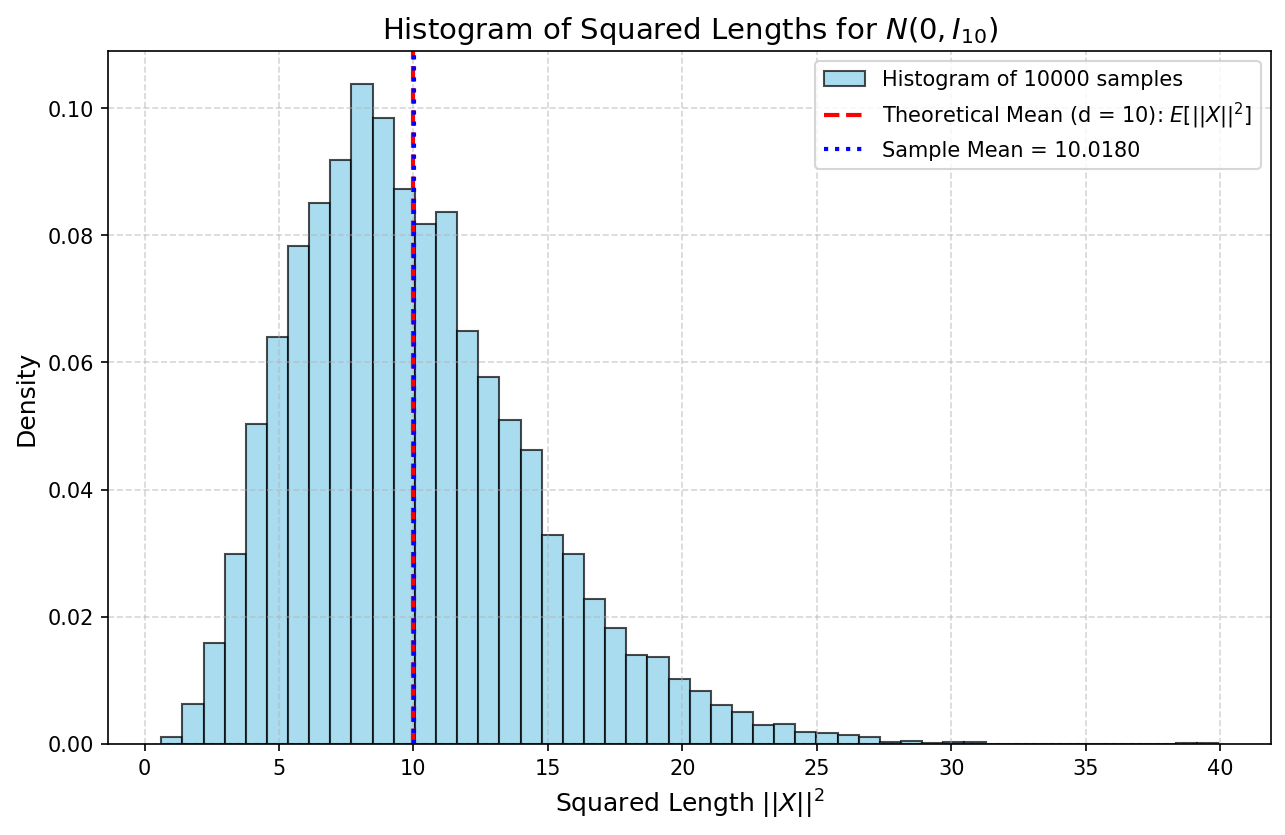
\includegraphics[width=\textwidth]{histogram_d10.png}
  \caption{Histogram of squared lengths for d=10. The distribution is centered near the theoretical mean of 10.}
\end{figure}

\subsubsection*{\normalfont}{$\therefore$ The typical (squared) length is approximately 10}

\subsubsection*{Graduate Level Explanation}
The random variable $Y = \|X\|^2$ for $X \sim N(0, I_d)$ follows a Chi-squared distribution, $Y \sim \chi^2(d)$. The expected value and variance are $\mathbb{E}[Y] = d$ and $\operatorname{Var}(Y) = 2d$. For $d=10$, this gives $\mathbb{E}[Y] = 10$ and $\operatorname{Var}(Y) = 20$. The histogram is a visualization of this $\chi^2(10)$ distribution, and its mode and mean are clearly clustered around the expected value of 10.

\subsubsection*{Learn Fast Explanation}
Imagine throwing darts at a 10-dimensional dartboard. The "squared length" is just the squared distance from the bullseye (the origin). While you might expect most darts to land near the center, in 10 dimensions they actually pile up around a specific distance. The "typical" squared distance isn't 0; it's 10. Our histogram shows this "pile-up" of squared distances, which is clearly centered at 10.

\noindent\rule{\textwidth}{0.4pt}\\

\newpage

%------------------
% Solution for 2(b)
%------------------
\subsection*{Solution 2}
\noindent\rule{\textwidth}{0.4pt}\\
\subsubsection*{Question 2 (b)}
\begin{flushleft}
    \textbf{Length concentration.} Write a procedure that draws 10000 points $X_1, \ldots, X_{10000}$ from the spherical Gaussian $N(0, I_d)$ and plots a histogram of their (squared) lengths $\|X_i\|^2$. 
    Repeat for $d=100$. Is the histogram more concentrated than in (a), or is it less concentrated? 
\end{flushleft}

\subsubsection*{Solution 2 (b)}
\subsubsection*{Python Code: d=100}
\begin{lstlisting}
import numpy as np
import matplotlib.pyplot as plt

# set dimension and number of samples
d = 100
num_samples = 10000
np.random.seed(42) 

# get 10000 points from N(0, I_d)
samples = np.random.normal(0, 1, size=(num_samples, d))

# calc the squared L2 norm for each point
squared_lengths_d100 = np.sum(samples**2, axis=1)

# calculate mean
sample_mean_d100 = np.mean(squared_lengths_d100)
print(f"Dimension (d): {d}")
print(f"Sample Mean of ||X||^2: {sample_mean_d100:.4f}")

# plot the histogram
plt.figure(figsize=(10, 6))
plt.hist(squared_lengths_d100, bins=50, color='skyblue', edgecolor='black', alpha=0.7, density=True,label=f'Histogram of {num_samples} samples')
plt.axvline(d, color='red', linestyle='--', linewidth=2, 
            label=f'Theoretical Mean (d = {d}): $E[||X||^2]$')
plt.axvline(sample_mean_d100, color='blue', linestyle=':', linewidth=2, 
            label=f'Sample Mean = {sample_mean_d100:.4f}')
# set plot args and save
plt.title('Histogram of Squared Lengths for $N(0, I_{100})$', fontsize=14)
plt.xlabel('Squared Length $||X||^2$', fontsize=12)
plt.ylabel('Density', fontsize=12)
plt.legend()
plt.grid(True, linestyle='--', alpha=0.5)
plt.savefig('histogram_d100.png', dpi=150, bbox_inches='tight')
\end{lstlisting}

\newpage
\subsection*{Solution 2}
\noindent\rule{\textwidth}{0.4pt}\\
\subsubsection*{Solution 2 (b)}
\subsubsection*{Plot}
\begin{figure}[h]
  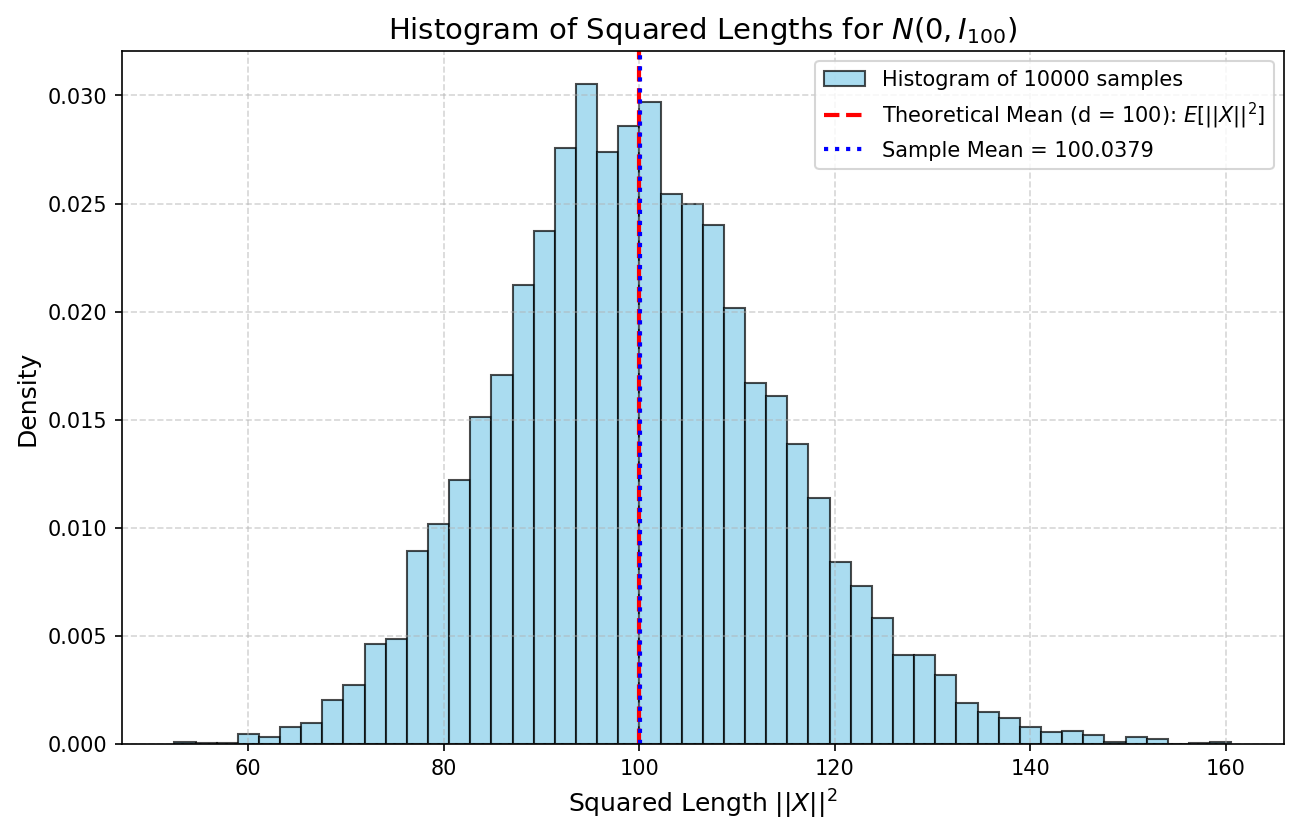
\includegraphics[width=\textwidth]{histogram_d100.png}
  \caption{Histogram of squared lengths for d=100. The distribution is much more sharply concentrated around its mean of 100.}
\end{figure}


\subsubsection*{Calculate Concentration}
To determine if the distribution is more concentrated, we must compare its relative spread. This is measured using the coefficient of variation or $CV$, which is defined as:
$$CV = \frac{\sigma}{\mu} \quad \text{ where } \quad \mu=d \text{ ,  } \sigma = \sqrt{2d}$$
For, $d=10$ and $d=100$, the coefficient of variation is:
$$CV_{10} = \frac{\sqrt{20}}{10} \approx 0.447\quad \text{ and }\quad CV_{100} = \frac{\sqrt{200}}{100} \approx 0.141$$
Hence, $CV_{100} < CV_{10}$ 

\subsubsection*{\normalfont}{$\therefore$ the distribution for $d=100$ is more concentrated than the distribution for $d=10$}

\subsubsection*{Graduate Level Explanation}
This demonstrates the phenomenon of **length concentration** in high dimensions. The coefficient of variation (CV) for the $\chi^2(d)$ distribution is $\text{CV} = \frac{\sqrt{\operatorname{Var}(Y)}}{\mathbb{E}[Y]} = \frac{\sqrt{2d}}{d} = \sqrt{\frac{2}{d}}$. This value scales as $O(1/\sqrt{d})$, meaning it approaches 0 as $d \to \infty$. Consequently, in high-dimensional spaces, the squared lengths of $N(0, I_d)$ vectors are not broadly distributed but instead concentrate in a "thin shell" very close to the expected value $d$.

\subsubsection*{Learn Fast Explanation}
Welcome to the "curse of dimensionality." On our 10-D dartboard, the squared distances were spread out (from $\approx 0$ to $25$). On the 100-D dartboard, the squared distances are centered at 100, but they are *packed* in a much tighter band (e.g., almost all are between 80 and 120). Relative to its mean of 100, this band is very narrow. This means in high dimensions, *all* "typical" points are about the same distance from the center—a very counter-intuitive but fundamental concept.

\noindent\rule{\textwidth}{0.4pt}\\

\newpage

%------------------
% Solution for 3
%------------------
\subsection*{Solution 3}
\noindent\rule{\textwidth}{0.4pt}\\
\subsubsection*{Question 3}
\begin{flushleft}
    Suppose $X \in \mathbb{R}^2$ has a Gaussian distribution with mean $\begin{bmatrix}1 \\ 2\end{bmatrix}$ and covariance matrix $\begin{bmatrix}2 & 0 \\ 0 & 4\end{bmatrix}$. 
    What is the distribution of the projection of $X$ onto direction $\frac{1}{\sqrt{2}}\begin{bmatrix}1 \\ 1\end{bmatrix}$? 
\end{flushleft}

\subsubsection*{Solution 3}
Let $X \sim N(\mu, \Sigma)$ where:
$$ \mu = \begin{bmatrix}1 \\ 2\end{bmatrix} \quad \quad \Sigma = \begin{bmatrix}2 & 0 \\ 0 & 4\end{bmatrix} \quad \quad v = \frac{1}{\sqrt{2}}\begin{bmatrix}1 \\ 1\end{bmatrix}$$

\begin{enumerate}
    \item Calculate the mean $\mu_Y$:
    \begin{align*}
    \mu_Y &= v^\top\mu \\
          &= \begin{bmatrix}1/\sqrt{2} & 1/\sqrt{2}\end{bmatrix} \begin{bmatrix}1 \\ 2\end{bmatrix} \\
          &= \left(\frac{1}{\sqrt{2}} \cdot 1\right) + \left(\frac{1}{\sqrt{2}} \cdot 2\right) \\
          &= \frac{1}{\sqrt{2}} + \frac{2}{\sqrt{2}} \\
          &= \frac{3}{\sqrt{2}}
    \end{align*}
    \item Calculate the variance $\sigma_Y^2$:
    \begin{align*}
        \sigma_Y^2 &= v^\top\Sigma v \\
        &= \begin{bmatrix}1/\sqrt{2} & 1/\sqrt{2}\end{bmatrix} \begin{bmatrix}2 & 0 \\ 0 & 4\end{bmatrix} \begin{bmatrix}1/\sqrt{2} \\ 1/\sqrt{2}\end{bmatrix} \\
        &= \begin{bmatrix}1/\sqrt{2} & 1/\sqrt{2}\end{bmatrix} \begin{bmatrix} 2 \cdot (1/\sqrt{2}) + 0 \\ 0 + 4 \cdot (1/\sqrt{2}) \end{bmatrix} \\
        &= \begin{bmatrix}1/\sqrt{2} & 1/\sqrt{2}\end{bmatrix} \begin{bmatrix} 2/\sqrt{2} \\ 4/\sqrt{2} \end{bmatrix} \\
        &= \left(\frac{1}{\sqrt{2}} \cdot \frac{2}{\sqrt{2}}\right) + \left(\frac{1}{\sqrt{2}} \cdot \frac{4}{\sqrt{2}}\right) \\
        &= \frac{2}{2} + \frac{4}{2} \\
        &= 1 + 2 = 3
    \end{align*}
\end{enumerate}

\subsubsection*{\normalfont}{$\therefore$ The distribution of the projection is $N\left(\frac{3}{\sqrt{2}}, 3\right)$.}
\subsubsection*{Graduate Level Explanation}
This result is a direct consequence of the affine transformation property of Gaussian vectors. If $X \sim N(\mu, \Sigma)$ and $Y = AX + b$, then $Y \sim N(A\mu + b, A\Sigma A^\top)$. In this problem, $A = v^\top$ and $b = 0$. This operation finds the 1-dimensional marginal distribution of the random vector $X$ along the axis defined by the vector $v$. Since the original covariance $\Sigma$ is diagonal, $X_1$ and $X_2$ are independent, but the projection $Y = \frac{1}{\sqrt{2}}(X_1 + X_2)$ is a sum of these independent variables, and its variance is the sum of their scaled variances.

\subsubsection*{Learn Fast Explanation}
Think of your 2D Gaussian $X$ as an oval-shaped cloud of 1,000s of data points, centered at $(1, 2)$. The oval is twice as wide in the $y$-direction (variance 4) as it is in the $x$-direction (variance 2). The "direction $v$" is just the 45-degree line $y=x$. Projecting the cloud onto this line is like shining a flashlight from behind the cloud and casting a shadow onto that 45-degree line. That shadow will also be a "cloud" of points, but it's 1-dimensional, so it's just a simple bell curve. Our calculation found the properties of that shadow-cloud: its center (mean) is at $3/\sqrt{2}$ ($\approx 2.12$) and its "spread" (variance) is $3$.

\noindent\rule{\textwidth}{0.4pt}\\

%------------------
% Solution for 4(a)
%------------------
\subsection*{Solution 4}
\noindent\rule{\textwidth}{0.4pt}\\
\subsubsection*{Question 4 (a)}
\begin{flushleft}
    We have three sensors $(X_1, X_2, X_3)$ whose joint distribution is Gaussian with mean zero and covariance matrix 
    \[
    \begin{bmatrix}
    6 & 3 & 1 \\
    3 & 9 & 0 \\
    1 & 0 & 2
    \end{bmatrix}
    \]
    What is the distribution of sensor $X_3$? 
\end{flushleft}

\subsubsection*{Solution 4 (a)}


\subsubsection*{\normalfont}{$\therefore$ }

\noindent\rule{\textwidth}{0.4pt}\\

\newpage

%------------------
% Solution for 4(b)
%------------------
\subsection*{Solution 4}
\noindent\rule{\textwidth}{0.4pt}\\
\subsubsection*{Question 4 (b)}
\begin{flushleft}
    We have three sensors $(X_1, X_2, X_3)$ whose joint distribution is Gaussian with mean zero and covariance matrix 
    \[
    \begin{bmatrix}
    6 & 3 & 1 \\
    3 & 9 & 0 \\
    1 & 0 & 2
    \end{bmatrix}
    \]
    What is the joint distribution of sensors $X_1, X_2$? 
\end{flushleft}

\subsubsection*{Solution 4 (b)}


\subsubsection*{\normalfont}{$\therefore$ }

\noindent\rule{\textwidth}{0.4pt}\\

\newpage

%------------------
% Solution for 4(c)
%------------------
\subsection*{Solution 4}
\noindent\rule{\textwidth}{0.4pt}\\
\subsubsection*{Question 4 (c)}
\begin{flushleft}
    We have three sensors $(X_1, X_2, X_3)$ whose joint distribution is Gaussian with mean zero and covariance matrix 
    \[
    \begin{bmatrix}
    6 & 3 & 1 \\
    3 & 9 & 0 \\
    1 & 0 & 2
    \end{bmatrix}
    \]
    Suppose we observe $X_2=2$ and $X_3=1$. 
    What is the resulting conditional distribution of $X_1$? 
\end{flushleft}

\subsubsection*{Solution 4 (c)}


\subsubsection*{\normalfont}{$\therefore$ }

\noindent\rule{\textwidth}{0.4pt}\\

\newpage

%------------------
% Solution for 5(a)
%------------------
\subsection*{Solution 5}
\noindent\rule{\textwidth}{0.4pt}\\
\subsubsection*{Question 5 (a)}
\begin{flushleft}
    \textbf{Modeling temperature data with Gaussian processes.} In this question, we will explore modeling of geospatial data via Gaussian processes. 
    Begin by downloading the files \texttt{gptrain.csv} and \texttt{gptest.csv} from the course webpage. 
    Each row in each file corresponds to a temperature reading at a given weather station in Brazil at 2 pm on January 1, 2021. The first column gives the latitude of the station, the second the longitude, and the final column is the temperature reading in degrees Celsius. 
    We will fit a simple Gaussian Process model on \texttt{gptrain.csv} and use it to infer temperatures at other locations at that same date and time. 
    We will fit a Gaussian process with covariance function 
    \[
    k(x, x') = \exp\left(\frac{-\|x-x'\|}{\sigma}\right)
    \]
    and mean function $m(x) = 20$ (degrees Celsius). 
    Here $\|x-x'\|$ denotes Euclidean distance between raw latitude and longitude coordinates. 
    Denote the locations in \texttt{gptrain.csv} by $X_{\text{tr}}$ and the temperatures at those locations by $y_{\text{tr}}$; 
    define $X_{\text{te}}, y_{\text{te}}$ analogously for \texttt{gptest.csv}. Thus $X_{\text{tr}}$ is a $93 \times 2$ matrix while $y_{\text{tr}}$ is a 93-dimensional vector. 
    
    The joint distribution of training and test responses can be written as 
    \[
    \begin{bmatrix} y_{\text{tr}} \\ y_{\text{te}} \end{bmatrix} \sim N\left(\begin{bmatrix} 20 \\ \vdots \\ 20 \end{bmatrix}, \begin{bmatrix} K_{\text{tr}} & K_{\text{tr,te}} \\ K_{\text{te,tr}} & K_{\text{te}} \end{bmatrix}\right)
    \]
    where the block matrix 
    \[
    \begin{bmatrix} K_{\text{tr}} & K_{\text{tr,te}} \\ K_{\text{te,tr}} & K_{\text{te}} \end{bmatrix}
    \]
    is the matrix arising from all pairwise evaluations of the covariance function $k(\cdot)$ over all training and testing locations, and its diagonal components $K_{\text{tr}}$ 
    and $K_{\text{te}}$ are the matrices arising from all pairwise covariances within the training and test sets, respectively. 
    Explain very briefly how the definition of Gaussian process allows us to come to this conclusion. 
\end{flushleft}

\subsubsection*{Solution 5 (a)}


\subsubsection*{\normalfont}{$\therefore$ }

\noindent\rule{\textwidth}{0.4pt}\\

\newpage

%------------------
% Solution for 5(b)
%------------------
\subsection*{Solution 5}
\noindent\rule{\textwidth}{0.4pt}\\
\subsubsection*{Question 5 (b)}
\begin{flushleft}
    \textbf{Modeling temperature data with Gaussian processes.} ... [Intro text from 5(a)  
    
    Define 
    \[
    m_{\text{te}} := \begin{bmatrix} 20 \\ \vdots \\ 20 \end{bmatrix} \in \mathbb{R}^{11}
    \]
    since there are 11 locations in the test set. 
    Using properties of the Gaussian, it can be shown that the distribution of test responses given training locations, training responses, and test locations, follows 
    \[
    y_{\text{te}} \mid y_{\text{tr}}, X_{\text{te}}, X_{\text{tr}} \sim m_{\text{te}} + N\left(K_{\text{te,tr}} \cdot K_{\text{tr}}^{-1}(y_{\text{tr}} - m_{\text{tr}}), K_{\text{te}} - K_{\text{te,tr}} K_{\text{tr}}^{-1} K_{\text{tr,te}}\right)
    \]
    In Bayesian language, this is the posterior predictive distribution. 
    \begin{itemize}
        \item Using $X_{\text{tr}}, X_{\text{te}}$, and $y_{\text{tr}}$, compute the posterior mean of $y_{\text{te}}$ via matrix multiplication, using $\sigma=1.5$ in the covariance function. 
        Report the mean squared error between your computed posterior mean and the true values found in $y_{\text{te}}$. 
        \item Report the mean squared error that you would have obtained by simply predicting the average value in $y_{\text{tr}}$ for all locations. 
    \end{itemize}
\end{flushleft}

\subsubsection*{Solution 5 (b)}

\subsubsection*{Python Code for Posterior Mean and MSE}
\begin{lstlisting}
import numpy as np
import pandas as pd
from scipy.spatial.distance import cdist
\end{lstlisting}

\subsubsection*{\normalfont}{$\therefore$ }

\noindent\rule{\textwidth}{0.4pt}\\

\newpage

%------------------
% Solution for 5(c)
%------------------
\subsection*{Solution 5}
\noindent\rule{\textwidth}{0.4pt}\\
\subsubsection*{Question 5 (c)}
\begin{flushleft}
    \textbf{Modeling temperature data with Gaussian processes.} 
    
    The diagonal of the posterior predictive matrix 
    \[
    K_{\text{te}} - K_{\text{te,tr}} K_{\text{tr}}^{-1} K_{\text{tr,te}}
    \]
    gives the conditional variances of the test responses given $X_{\text{tr}}, X_{\text{te}}$, and $y_{\text{tr}}$. 
    \begin{itemize}
        \item Create a rich grid (at least 5000 points) of test latitudes and longitudes within the range found in the training set. 
        Make a plot showing the predicted (posterior mean) temperature at all points in the grid. 
        You might find the function \texttt{matplotlib.pyplot.imshow} helpful for this. 
        \item Make another plot showing the standard deviation of the prediction at all points in the grid. 
        Plot the locations of the stations found in the training set as well. 
        \item What do you notice about the relationship of the standard deviation of the prediction and the distance of that prediction to a training point? 
    \end{itemize}
\end{flushleft}

\subsubsection*{Solution 5 (c)}

\subsubsection*{Python Code for Grid Predictions and Plots}
\begin{lstlisting}
import numpy as np
import pandas as pd
import matplotlib.pyplot as plt
from scipy.spatial.distance import cdist
\end{lstlisting}

\begin{comment}
\begin{figure}[h]
  \includegraphics[width=\textwidth]{gp_mean_plot.png}
  \caption{Posterior Mean Temperature Grid}
\end{figure}
\begin{figure}[h]
  \includegraphics[width=\textwidth]{gp_std_plot.png}
  \caption{Posterior Standard Deviation Grid}
\end{figure}
\end{comment}

\subsubsection*{\normalfont}{$\therefore$ }

\noindent\rule{\textwidth}{0.4pt}\\

\newpage

%------------------
% Solution for 6(a)
%------------------
\subsection*{Solution 6}
\noindent\rule{\textwidth}{0.4pt}\\
\subsubsection*{Question 6 (a)}
\begin{flushleft}
    \textbf{Four friends} $F_1, F_2, F_3, F_4$ like going to the movies. 
    When a new movie comes out, they behave according to the following scheme: 
    \begin{itemize}
    \item $F_1$ sees the movie with probability 0.5. 
    \item $F_2$ sees the movie with probability 0.7, independently. 
    \item If either of $F_1$ or $F_2$ (or both) see the movie, $F_3$ goes to see it with probability 0.8; 
    if neither $F_1$ nor $F_2$ sees the movie, $F_3$ sees it with probability 0.3. 
    \item If $F_3$ sees the movie, then $F_4$ goes to see it with probability 0.9. 
    If $F_3$ doesn't see the movie, then $F_4$ sees it with probability 0.5. 
    \end{itemize}

    Let $F_1, F_2, F_3, F_4 \in \{0,1\}$ denote who sees the movie. 
    The dependencies between these four random variables can be captured by the following directed graph: 

    \begin{center}
    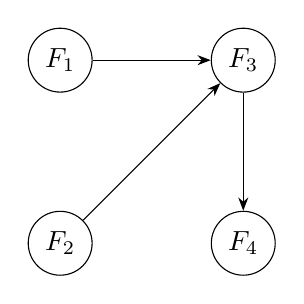
\begin{tikzpicture}[node distance=1.5cm]
        \node[circle, draw] (F1) {$F_1$}; 
        \node[circle, draw, below=of F1] (F2) {$F_2$}; 
        \node[circle, draw, right=of F1] (F3) {$F_3$};
        \node[circle, draw, below=of F3] (F4) {$F_4$};
        \draw[-Stealth] (F1) -- (F3); 
        \draw[-Stealth] (F2) -- (F3); 
        \draw[-Stealth] (F3) -- (F4); 
    \end{tikzpicture}
    \end{center}

    Give the conditional probability tables for this Bayes net. 
\end{flushleft}

\subsubsection*{Solution 6 (a)}


\subsubsection*{\normalfont}{$\therefore$ }

\noindent\rule{\textwidth}{0.4pt}\\

\newpage

%------------------
% Solution for 6(b)
%------------------
\subsection*{Solution 6}
\noindent\rule{\textwidth}{0.4pt}\\
\subsubsection*{Question 6 (b)}
\begin{flushleft}
    \textbf{Four friends} ... [Intro text from 6(a)  

    \begin{center}
    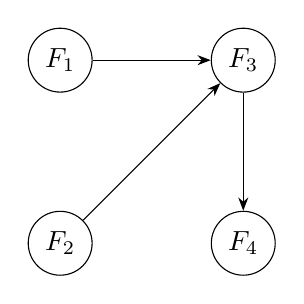
\begin{tikzpicture}[node distance=1.5cm]
        \node[circle, draw] (F1) {$F_1$}; 
        \node[circle, draw, below=of F1] (F2) {$F_2$}; 
        \node[circle, draw, right=of F1] (F3) {$F_3$};
        \node[circle, draw, below=of F3] (F4) {$F_4$};
        \draw[-Stealth] (F1) -- (F3); 
        \draw[-Stealth] (F2) -- (F3); 
        \draw[-Stealth] (F3) -- (F4); 
    \end{tikzpicture}
    \end{center}

    What is the probability of the configuration $F_1 = F_2 = F_3 = 1, F_4 = 0$? 
\end{flushleft}

\subsubsection*{Solution 6 (b)}


\subsubsection*{\normalfont}{$\therefore$ }

\noindent\rule{\textwidth}{0.4pt}\\

\newpage

%------------------
% Solution for 7
%------------------
\subsection*{Solution 7}
\noindent\rule{\textwidth}{0.4pt}\\
\subsubsection*{Question 7}
\begin{flushleft}
    \textbf{Non-uniqueness of underlying DAG.} Suppose random variables $X$ and $Y$ take values in $\{0,1\}$. 
    Does the joint distribution of $(X, Y)$ necessarily factor over the DAG on the left below? 
    What about the DAG on the right? 

    \begin{center}
    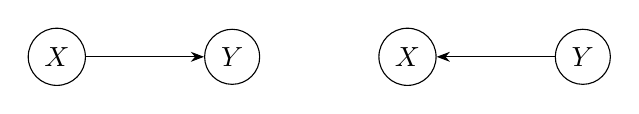
\begin{tikzpicture}[node distance=1.5cm]
        \node[circle, draw] (F1) {$X$}; 
        \node[circle, draw, right=of F1] (F3) {$Y$}; 
        \node[circle, draw, right=of F3] (F2) {$X$};
        \node[circle, draw, right=of F2] (F4) {$Y$};
        \draw[-Stealth] (F1) -- (F3); 
        \draw[-Stealth] (F4) -- (F2); 
    \end{tikzpicture}
    \end{center}
\end{flushleft}

\subsubsection*{Solution 7}


\subsubsection*{\normalfont}{$\therefore$ }

\noindent\rule{\textwidth}{0.4pt}\\

\newpage

%------------------
% Solution for 8(a)
%------------------
\subsection*{Solution 8}
\noindent\rule{\textwidth}{0.4pt}\\
\subsubsection*{Question 8 (a)}
\begin{flushleft}
    \textbf{Genes, diseases, and outcomes.} There is a fictitious disease $(D)$ that can cause paralysis $(P)$. 
    Whether or not an individual gets this disease depends in large part on two genes, $G_1$ and $G_2$. 
    Here is a summary: 

    \begin{itemize}
    \item Each of these genes $G_1, G_2$ can either be normal (also known as wild-type), represented by $G_i=0$, or mutant, represented by $G_i=1$. 
    \item For a person with $G_1=G_2=0$ (both genes wild-type) the probability of acquiring the disease is zero. 
    If $G_1$ is mutant and $G_2$ is wild-type, the probability is 0.2. 
    If $G_1$ is wild-type and $G_2$ is mutant, it is 0.1. 
    And if both genes are mutant, then the disease probability is 0.5. 
    \item For an individual with the disease, the probability of paralysis is 0.5. 
    Without the disease, there is still a small probability of paralysis (from other causes): 0.01. 
    \item $G_1$ is mutant with probability 0.1 and $G_2$ is mutant with probability 0.2; these are independent. 
    \end{itemize}

    Draw a suitable Bayes net over the variables $G_1, G_2, D, P$, and give all relevant conditional probability tables. 
    Let $D=1$ if the disease is present and $D=0$ if it isn't; likewise with paralysis. 
\end{flushleft}

\subsubsection*{Solution 8 (a)}

\subsubsection*{Bayes Net Diagram}
\begin{comment}
    \begin{center}
    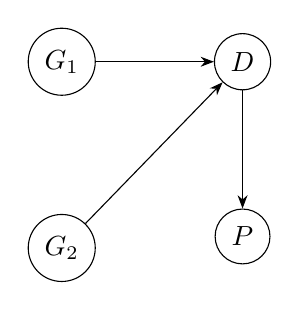
\begin{tikzpicture}[node distance=1.5cm]
        \node[circle, draw] (G1) {$G_1$};
        \node[circle, draw, below=of G1] (G2) {$G_2$};
        \node[circle, draw, right=of G1] (D) {$D$};
        \node[circle, draw, below=of D] (P) {$P$};
        \draw[-Stealth] (G1) -- (D);
        \draw[-Stealth] (G2) -- (D);
        \draw[-Stealth] (D) -- (P);
    \end{tikzpicture}
    \end{center}
\end{comment}

\subsubsection*{Conditional Probability Tables}


\subsubsection*{\normalfont}{$\therefore$ }

\noindent\rule{\textwidth}{0.4pt}\\

\newpage

%------------------
% Solution for 8(b)
%------------------
\subsection*{Solution 8}
\noindent\rule{\textwidth}{0.4pt}\\
\subsubsection*{Question 8 (b)}
\begin{flushleft}
    \textbf{Genes, diseases, and outcomes.} ... [Intro text from 8(a)  

    What is the probability of disease $(D=1)$? 
\end{flushleft}

\subsubsection*{Solution 8 (b)}


\subsubsection*{\normalfont}{$\therefore$ }

\noindent\rule{\textwidth}{0.4pt}\\

\newpage

%------------------
% Solution for 8(c)
%------------------
\subsection*{Solution 8}
\noindent\rule{\textwidth}{0.4pt}\\
\subsubsection*{Question 8 (c)}
\begin{flushleft}
    \textbf{Genes, diseases, and outcomes.} ... [Intro text from 8(a)  

    What is the probability of paralysis $(P=1)$? 
\end{flushleft}

\subsubsection*{Solution 8 (c)}


\subsubsection*{\normalfont}{$\therefore$ }

\noindent\rule{\textwidth}{0.4pt}\\

\newpage

%------------------
% Solution for 8(d)
%------------------
\subsection*{Solution 8}
\noindent\rule{\textwidth}{0.4pt}\\
\subsubsection*{Question 8 (d)}
\begin{flushleft}
    \textbf{Genes, diseases, and outcomes.} ... [Intro text from 8(a)  

    We observe that a person has paralysis. What is the probability that they have the disease? 
\end{flushleft}

\subsubsection*{Solution 8 (d)}


\subsubsection*{\normalfont}{$\therefore$ }

\noindent\rule{\textwidth}{0.4pt}\\

\newpage

%------------------
% Solution for 8(e)
%------------------
\subsection*{Solution 8}
\noindent\rule{\textwidth}{0.4pt}\\
\subsubsection*{Question 8 (e)}
\begin{flushleft}
    \textbf{Genes, diseases, and outcomes.} ... [Intro text from 8(a)  

    We observe that a person has the disease $(D=1)$. 
    What is the probability that they have the mutant form of gene $G_1$? 
\end{flushleft}

\subsubsection*{Solution 8 (e)}


\subsubsection*{\normalfont}{$\therefore$ }

\noindent\rule{\textwidth}{0.4pt}\\

\newpage

%------------------
% Solution for 9(a)
%------------------
\subsection*{Solution 9}
\noindent\rule{\textwidth}{0.4pt}\\
\subsubsection*{Question 9 (a)}
\begin{flushleft}
    \textbf{A character-level RNN for text generation.} Download the file \texttt{rnn-gen.zip} from the course webpage; 
    it contains a Jupyter notebook, \texttt{text-gen-rnn.ipynb}, as well as data and helper files. 
    The notebook is adapted from an excellent blog post by Andrej Karpathy, \textit{The unreasonable effectiveness of recurrent neural networks}. 
    It fits an RNN (more precisely, an LSTM) to the text of Shakespeare's plays and then uses this to generate more text, one character at a time. 
    Work through the notebook and try to understand what is going on. There are just three small questions to answer. 
    
    How many characters are we considering, and what is the integer code for 'A'? 
\end{flushleft}

\subsubsection*{Solution 9 (a)}


\subsubsection*{\normalfont}{$\therefore$ }

\noindent\rule{\textwidth}{0.4pt}\\

\newpage

%------------------
% Solution for 9(b)
%------------------
\subsection*{Solution 9}
\noindent\rule{\textwidth}{0.4pt}\\
\subsubsection*{Question 9 (b)}
\begin{flushleft}
    \textbf{A character-level RNN for text generation.} ... [Intro text from 9(a)  

    What is the length of the corpus in characters? 
\end{flushleft}

\subsubsection*{Solution 9 (b)}


\subsubsection*{\normalfont}{$\therefore$ }

\noindent\rule{\textwidth}{0.4pt}\\

\newpage

%------------------
% Solution for 9(c)
%------------------
\subsection*{Solution 9}
\noindent\rule{\textwidth}{0.4pt}\\
\subsubsection*{Question 9 (c)}
\begin{flushleft}
    \textbf{A character-level RNN for text generation.} ... [Intro text from 9(a)  

    The input and output size for the RNN are set to 66. Why is this? 
\end{flushleft}

\subsubsection*{Solution 9 (c)}


\subsubsection*{\normalfont}{$\therefore$ }

\noindent\rule{\textwidth}{0.4pt}\\

\end{document}
